\section{Conclusiones} \label{sec:conclusiones}


En este trabajo se ha estudiado el rendimiento de tres arquitecturas de redes neuronales convolucionales, \textit{EEGNet}, \textit{DeepConvNet} y \textit{ShallowConvNet}, para la clasificación de señales EEG asociadas a las tareas estática y de movimiento durante el uso de un exoesqueleto. Asimismo, se han comparado cuatro estrategias de entrenamiento: \textit{Intra-Sesión}, \textit{Inter-Sesión}, \textit{Inter-Usuarios} y \textit{Continuo}.

Hay estudios que señalan que el rendimiento de los modelos de DeepLearning para \acrshort{eeg} depende en gran medida del conjunto de datos, del paradigma experimental y de la estrategia de entrenamiento utilizada. Por este motivo es difícil establecer una arquitectura o un método de entrenamiento que sea superior en todas las aplicaciones, sino que debe evaluarse bajo las condiciones concretas de cada problema \cite{kollod_DeepComparisons2023}.

Los resultados obtenidos muestran, de manera general, que la arquitectura, la tarea analizada y el usuario tienen una mayor influencia sobre el rendimiento que el método de entrenamiento. Aunque se observan diferencias entre las estrategias de entrenamiento, estas no se mantienen de forma consistente entre todas las arquitecturas, tareas y participantes.

\subsection{Influencia de la arquitectura}

La arquitectura \textit{ShallowConvNet} presenta el mejor rendimiento global, con una precisión media aproximada del 76.6\%. \textit{EEGNet} obtiene un resultado intermedio, cercano al 71.4\%, mientras que \textit{DeepConvNet} alcanza la precisión media más baja, con aproximadamente un 69.4\%.

La superioridad de \textit{ShallowConvNet} se mantiene entre las dos tareas y los diferentes métodos de entrenamiento. Además, esta arquitectura muestra un comportamiento relativamente estable frente a los cambios de configuración, aunque presenta una variabilidad considerable entre usuarios.

Por su parte, \textit{EEGNet} obtiene resultados intermedios en la mayoría de las configuraciones. El estar orientado a diferentes paradigmas BCI puede favorecer su capacidad de generalización, aunque la escasez del conjunto de datos utilizado en este estudio puede hacer que esta arquitectura no alcance el rendimiento esperado.

\textit{DeepConvNet} presenta generalmente los peores resultados y una mayor reducción de precisión en la tarea de movimiento. Una posible explicación es que su mayor número de parámetros requiera una mayor cantidad de datos para aprender y generalizar a nuevas observaciones. Es posible que esta arquitectura no haya podido obtener el rendimiento esperado debido al número limitado de participantes y sesiones disponibles,

Sin embargo, también hay que tener en cuenta que se ha utilizado una configuración de hiperparámetros común en todos los experimentos. Aunque esta decisión permite reducir la complejidad del estudio, puede favorecer a determinados modelos, ya que cada arquitectura podría requerir una configuración específica para obtener su rendimiento óptimo.

A falta de una búsqueda de parámetros exhaustiva, los resultados indican que la elección de la arquitectura tiene una influencia más evidente que la elección del método de entrenamiento.

\subsection{Influencia de la tarea}

La tarea estática alcanza una precisión media global aproximada del 76.0\%, mientras que la tarea de movimiento obtiene un valor cercano al 69.1\%. Esto supone una diferencia media de aproximadamente siete puntos porcentuales a favor de la tarea estática.

La mayoría de configuraciones de arquitecturas, métodos de entrenamiento y usuarios analizados presentan una mayor precisión en la tarea estática. Por tanto, los resultados indican que la tarea de movimiento presenta una mayor dificultad de generalización.

Una posible explicación es que los patrones EEG asociados a la tarea de movimiento sean más variables o menos diferenciables que los relacionados con la tarea estática. Los posibles factores que pueden contribuir a esta diferencia son: el cambio en la concentración de los participantes, la presencia de artefactos o las características concretas del protocolo de adquisición.

Sin embargo, los resultados obtenidos no permiten determinar cuál de estos factores es el responsable de la diferencia observada. Para ello sería necesario realizar un análisis más específico de las señales y de las condiciones experimentales de cada tarea.

\subsection{Variabilidad entre usuarios}

El propio usuario se presenta como uno de los factores con mayor influencia sobre los resultados. La desviación estándar de las precisiones medias de los participantes alcanza los 9.15 puntos porcentuales, mientras que el rango de medias globales va desde aproximadamente un 61.6\% para el \textbf{usuario 2} hasta un 81.3\% para el \textbf{usuario 4}, lo que supone una diferencia cercana a 20 puntos porcentuales entre ambos. Esta dispersión es superior a la observada entre los métodos de entrenamiento y sugiere una importante dependencia del rendimiento respecto al participante.

Además, el comportamiento de los usuarios no presenta una tendencia general. Por ejemplo, el \textbf{usuario 1} obtiene los mejores resultados en la tarea estática, mientras que el \textbf{usuario 4} presenta el mejor rendimiento en la tarea de movimiento. Aunque, en general, la precisión de la tarea estática supera a la de movimiento en aproximadamente 7 puntos, esta diferencia no se observa de la misma forma en todos los participantes. El \textbf{usuario 2}, por ejemplo, mejora 3 puntos porcentuales en la tarea de movimiento, mientras que el \textbf{usuario 3} experimenta una reducción cercana a 20 puntos.

Estas diferencias pueden estar relacionadas con la variabilidad fisiológica de las señales EEG, la calidad del registro, la colocación de los electrodos, la capacidad de concentración o la forma en que cada participante ejecuta las tareas. El hecho de que el orden relativo de los usuarios cambie entre tareas indica que no todos los participantes se ven afectados de la misma manera por la complejidad de la tarea.

En conjunto, los resultados muestran una elevada variabilidad inter-sujeto.


\subsection{Influencia de los métodos de entrenamiento}

El método \textit{Inter-Sesión} obtiene la mayor precisión media global, con aproximadamente un 74.8\%. Después va el entrenamiento \textit{Inter-Usuarios}, con un 72.9\%, seguido del entrenamiento \textit{Continuo}, con un 71.4\%, y del entrenamiento \textit{Intra-Sesión}, con un 70.4\%.

El menor rendimiento del método \textit{Intra-Sesión} era de esperar, ya que al utilizar datos de un único día y usuario, el modelo dispone de menos ejemplos para aprender y generalizar. Además puede presentar una mayor dependencia de las características particulares de esa sesión.

El método \textit{Inter-Sesión} puede aprovechar información de sesiones anteriores del mismo usuario, lo que permite aumentar la cantidad de datos de entrenamiento. Además, al centrarse en un único participante, el modelo no se enfrenta a la variabilidad asociada a otros usuarios. Esto podría explicar su mayor precisión media y su menor desviación.

Los entrenamientos \textit{Inter-Usuarios} y \textit{Continuo} no presentan una mejora claramente diferenciada respecto al entrenamiento \textit{Intra-Sesión}. Esto quiere decir que el uso de un modelo inicial entrenado con otros usuarios no garantiza un aumento de la precisión tras su adaptación al usuario objetivo.

Una posible explicación es que, las características compartidas entre participantes sean limitadas y que el conocimiento adquirido con otros usuarios no pueda transferirse directamente. También es posible que, durante la adaptación individual, el modelo modifique parte de los pesos generales aprendidos sin disponer todavía de suficientes datos del usuario objetivo, perdiendo así información relevante. Queda por determinar si una modificación en el modelo general o en el proceso de \textit{fine-tuning} puede mejorar el rendimiento del modelo específico.

En cualquier caso, los resultados no permiten establecer un método de entrenamiento claramente superior. Aunque \textit{Inter-Sesión} presenta el mejor rendimiento medio, no presenta la misma mejora en todas las arquitecturas, tareas y usuarios. Esto no implica que los métodos sean equivalentes. Los resultados pueden indicar que sus diferencias son menores que las producidas por los otros factores.

\subsection{Conclusión general}

En general, se puede concluir que \textit{ShallowConvNet} es la arquitectura más adecuada para este conjunto de datos, al presentar la mayor precisión media y un comportamiento comparativamente estable entre tareas y métodos de entrenamiento.

También se observa una diferencia clara entre las dos tareas estudiadas. La tarea estática obtiene mejores resultados que la tarea de movimiento de manera consistente, aunque no se puede obtener una razón concreta de esta diferencia a partir de los resultados obtenidos.

En cuanto a las estrategias de entrenamiento, \textit{Inter-Sesión} presenta los mejores resultados medios, pero la mejora respecto a los demás métodos no es consistente. Los métodos que incorporan información de otros usuarios no consiguen una ventaja suficientemente grande como para justificar la mayor complejidad en su proceso de entrenamiento.

En las condiciones evaluadas, aumentar la complejidad de la estrategia de entrenamiento equivale necesariamente a una mejora proporcional de la precisión. La arquitectura seleccionada y las características particulares del usuario y de la tarea parecen ser factores más determinantes.

Finalmente, la elevada variabilidad entre usuarios sugiere que la capacidad de generalización de los modelos está extremadamente condicionada por las características individuales de las señales EEG. Esto puede dificultar la elección de una configuración óptima de arquitectura y método de entrenamiento que sea válida para todos los participantes.

  {
    \begin{comment}


    Este apartado introductorio faltaría rellenarlo con las conclusiones obtenidas a partir de los resultados del capítulo anterior.




    ShallowConvNet suele ser el mejor.

    DeepConvNet normalmente el peor.

    Static funciona mejor que Motion.

    Hay bastante dependencia del usuario.

    Inter-Sesión e Inter-Users mejoran ligeramente respecto a Intra.

    Continuous no supone una mejora espectacular.

    Me queda realmente poco, comentar los resultados y las conclusiones. Viendo las gráficas se queda algo así:

    ShallowConvNet suele ser el mejor. (global Avg= 0.76)
    EEGNet Suele mantenerse en el medio (global Avg = 0.71)
    DeepConvNet normalmente el peor. (global Avg = 0.69)
    model\_name         avg\_acc1
    varchar            double

    ShallowConvNet  0.7662446249402762
    DeepConvNet     0.6937626027609743
    EEGNet          0.7137599206349203

    Static funciona mejor que Motion.
    task\_mode       avg\_acc1
    varchar         double

    motion     0.6906362007168463
    static     0.7598059064895796


    Hay bastante dependencia del usuario.
    user        avg\_acc1
    int64        double

    0  0.6762566137566141
    1  0.7917231766124173
    2   0.615861618798956
    3  0.7458137100994237
    4  0.8133346823148518


    Inter-Sesión e Inter-Users mejoran ligeramente respecto a Intra.

    training\_method       avg\_acc1
    varchar            double

    trainingA        0.7044462481962481  -> intrasesión
    trainingB        0.7478039759593151  -> inter sesiones
    trainingC        0.7294351951306842  -> inter users
    trainingD         0.713930348258706  -> continuous



    Continuous no supone una mejora espectacular.

    Solo habría que argumentarlos o dar una hipótesis.
    En el caso de los métodos de las arquitecturas se pueden argumentar ligeramente con estas frases:
    EEGNet, es agnóstico al paradigma BCI, por lo que sus resultados pueden ser buenos, pero al no estar optimizada para MRCP puede quedarse atrás.

    DeepConvNet y ShallowConvNet sí fueron entrenados y diseñados con datos MRCP (l1 = Hand Left, l2 = Hand Right,  l3 = Feet, l4 = Rest)
    En el paper original DeepConvNet obtiene ligeramente peores resultados que ShallowConvNet en varios datasets (-5\%). La diferencia observada en este estudio (-10\%) puede atribuirse a que DeepConvNet, al tener un mayor número de parámetros entrenables, requiere a su vez más cantidad de datos para poder generalizar correctamnete. Debido a la limitada cantidad de datos utilizados en este estudio (5 usuarios y 5 sesiones), el rendimiento de DeepConvNet suele ser peor.

    Las tereas:
    motion suele tener más ``ruido mental'', suele ser más dificil concentrarse moverse, y suele ser mas complejo diferenciarlo en las señales.
    static en cambio suele sér más sencillo.

    Los entrenamientos:
    Se puede estipular que intra-sesion tiene muy pocos datos y que no es capaz de generalizar.
    Inter-sesiónes, tiene más datos que intra sesión. Además aprende de manera iterativa, al utilizar los datos de las sesiones anteriores, los modelos finales aprenden correctamente los patrones que se han visto en las sesiones anteriores, además el centrarse en un unico usuario no se enfrenta al problema de la variabilidad entre ellos.
    Continious y inter Users: se puede estipular que el añadir los datos de todos los usuarios y todas las sesiones puede hacer que aprenda correctamente datos globales, pero que al entrenar individualmente con los datos de cada usuario pierda el conocimiento que aprendió con los datos de otros usuarios.


    Esta ausencia de una ventaja sistemática no implica que los métodos produzcan resultados equivalentes, sino que, con los datos disponibles, sus diferencias quedan parcialmente ocultas por otros factores de mayor influencia, como la arquitectura seleccionada y la variabilidad entre sujetos.

    En conjunto, la elevada variabilidad entre los usuarios  puede dificultar la mejora en los resultados por los métodos de entrenamiento. Las diferencias fisiológicas, la calidad de las señales registradas y la capacidad de cada participante para realizar la tarea pueden producir variaciones superiores al efecto del propio método.

    Por tanto, para la tarea estática, la arquitectura utilizada tiene un efecto más visible sobre la precisión que el método de entrenamiento.

    Esta modificación del orden relativo de los usuarios sugiere que la dificultad de la tarea depende también de las características particulares de cada sujeto.

    Las diferencias entre usuarios vuelven a superar, en numerosos casos, las observadas entre métodos de entrenamiento. Este comportamiento sugiere que la capacidad de generalización de los modelos está condicionada por la variabilidad de las señales EEG individuales, especialmente en la tarea de movimiento.

    No obstante, a partir de este análisis descriptivo no puede determinarse por sí solo si esta diferencia se debe a una mayor complejidad fisiológica de la tarea, a las características del protocolo experimental o a diferencias en la calidad de las señales registradas.


    Por tanto, los resultados obtenidos no respaldan la existencia de un método de entrenamiento universalmente superior. La estrategia utilizada parece tener un efecto secundario frente a otros factores, especialmente la arquitectura, la tarea y la identidad del usuario. También es posible que el reducido número de sujetos y sesiones limite la capacidad del análisis para detectar diferencias moderadas entre métodos.

    Esta falta de diferencias constituye en sí misma un resultado relevante: dentro de las condiciones experimentales estudiadas, aumentar la complejidad del procedimiento de entrenamiento no se traduce necesariamente en una mejora proporcional del rendimiento.

    Los métodos de entrenamiento
    \end{comment}
  }

\subsection{Trabajos futuros}

\subsubsection{Maquina de estados finitos}

Una posible línea de trabajo futuro consiste en integrar dos modelos distintos dentro de un mismo sistema de control, con el objetivo de aprovechar las dos tareas de imaginación motora para construir una \acrshort{bci} de bucle cerrado basada en una máquina de estados finitos. Este enfoque permitiría controlar de forma independiente el comportamiento del exoesqueleto y proporcionar al usuario un mayor grado de autonomía durante la interacción.

En este planteamiento, el sistema comenzaría en un estado de \textbf{parada}, en el que el exoesqueleto permanecería inmóvil mientras un modelo entrenado sobre la tarea estática (\textit{Modelo de Inicio de la Marcha}) monitoriza continuamente la actividad cerebral del usuario. Cuando dicho modelo detectase una intención de inicio de la marcha, el sistema realizaría una transición al estado de \textbf{movimiento}.

Durante este segundo estado, el exoesqueleto ejecutaría la marcha asistida mientras un modelo entrenado sobre la tarea en movimiento (\textit{Modelo de Detención}) analiza la señal EEG en busca de una intención de parada. Una vez detectada esta intención, el sistema regresaría al estado de \textbf{parada}, completando así el ciclo de control.

Con el objetivo de reducir la probabilidad de falsos positivos, las predicciones de ambos modelos podrían combinarse mediante una estrategia basada en una media ponderada. De esta forma, aunque cada estado disponga de un clasificador principal, la decisión final tendría en cuenta la información proporcionada por ambos modelos, aumentando potencialmente la robustez del sistema frente a errores de clasificación.

La Figura \ref{fig:diagrama_estados} muestra una representación conceptual de esta máquina de estados finitos y de las transiciones asociadas a cada uno de los modelos de clasificación.

\begin{figure}[htbp]
  \centering
  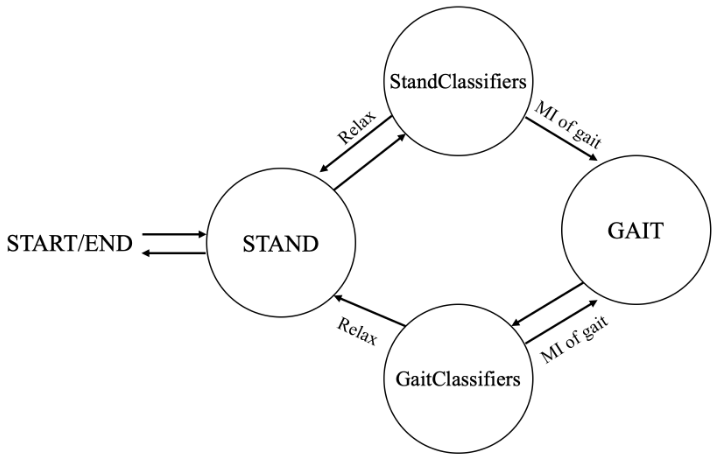
\includegraphics[width=0.90\textwidth]{img/diagrama_estados_ferrero.png}
  %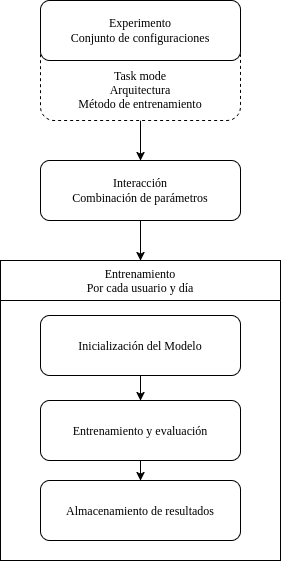
\includegraphics[height=\dimexpr\pagegoal-\pagetotal-\baselineskip\relax,width=\textwidth,keepaspectratio]{img/diagrama_pipeline.drawio.png}
  \caption{Ejemplo de arquitectura de control basada en una máquina de estados finitos para sistemas BCI. Tomado de \cite{ferrero_BMIBased2021}}
  \label{fig:diagrama_estados}
\end{figure}

Este procedimiento es consistente con diversas propuestas presentes en la literatura, donde el control de sistemas \acrshort{bci} se aborda mediante máquinas de estados finitos donde varios clasificadores de EEG son utilizados para detectar las distintas intenciones del usuario, tales como iniciar, mantener, o finalizar la marcha. En esta línea, Ferrero et al. \parencite{ferrero_BMIBased2021} emplean una arquitectura de control basada en estados para gobernar la marcha de un exoesqueleto, mientras que los mismos autores \parencite{ferrero_BCIBased2021} aplican un enfoque similar al control de una cinta de marcha.

Asimismo, \textcite{choi_DevelopingMotor2020} demostraron la viabilidad de este paradigma en sistemas de control asíncronos para exoesqueletos de miembro inferior, utilizando tres estados funcionales (parada, marcha y sentado) y transiciones activadas mediante imaginación motora.

\subsubsection{Interpretabilidad de los modelos utilizados}

Otra posible línea de investigación consiste en estudiar la interpretabilidad de los modelos entrenados. Tanto \textcite{lawhern_EEGNetCompact2018} como \textcite{schirrmeister_DeepLearning2017} aplicaron estas técnicas para analizar las características aprendidas por las arquitecturas propuestas en sus respectivos trabajos.

Un análisis interpretable permitiría determinar qué componentes de la señal tienen una mayor influencia en la clasificación de cada una de las tareas propuestas. En particular, podría estudiarse la relevancia de los distintos electrodos y regiones espaciales o las de distintas bandas de frecuencia e intervalos temporales.

Este análisis permitiría comprobar si los modelos basan sus decisiones en patrones neurofisiológicos comunes o si, por el contrario, dependen en exceso de artefactos o características particulares del conjunto de datos. Además, la comparación de los patrones aprendidos por \textit{EEGNet}, \textit{DeepConvNet} y \textit{ShallowConvNet} ayudaría a explicar las diferencias de rendimiento observadas entre las arquitecturas.

\subsubsection{Evaluación de la cantidad de datos necesaria}

En los experimentos realizados se utilizaron para el entrenamiento los ocho primeros ensayos de cada día, de un total de once. Esto representa aproximadamente un 73\% de los ensayos disponibles, mientras que los tres restantes se reservaron para la evaluación.

Como trabajo futuro, sería interesante estudiar cómo varía el rendimiento de las arquitecturas al modificar la cantidad de información utilizada durante el entrenamiento. Para ello, podrían entrenarse los modelos utilizando una cantidad diferente de ensayos, pudiendo mantener un conjunto de evaluación común para garantizar que los resultados obtenidos sean comparables.

Este análisis permitiría observar la relación entre la cantidad de datos disponibles y la precisión alcanzada, así como identificar el punto a partir del cual la incorporación de nuevos ensayos no produce grandes mejoras.

También permitiría estimar la cantidad mínima de información necesaria para adaptar un modelo a un nuevo usuario, reduciendo el tiempo de calibración.Esto resulta especialmente relevante para el desarrollo de sistemas \acrshort{bci}, ya que una estrategia capaz de alcanzar un rendimiento adecuado con pocos ensayos facilitaría su adopción por parte de nuevos usuarios y reduciría el tiempo de aprendizaje.